\documentclass[18pt]{beamer}
\usepackage[utf8]{inputenc}
\usepackage{templates/mytemplate}
\usepackage{graphicx}
\usepackage{microtype}
\usepackage{listings}
\usepackage{xcolor}
\usepackage{siunitx}
\usepackage{physics}

\hypersetup{colorlinks, linkcolor=black, urlcolor=kit-blue100}
\lstset{
  basicstyle=\ttfamily,
  basicstyle=\footnotesize,
  language=C++,
}

\newcommand\pro{\item[$\oplus$]}
\newcommand\con{\item[$\ominus$]}

\title{Track Quality Estimation for CDC (local) Tracking}
\subtitle{}
\author{Michael Eliachevitch}
\date{10 February 2018}
\titleimage{transparent}
\institute{ETP - KIT}

\begin{document}
\selectlanguage{english}

% \begin{frame}
%   \titlepage
% \end{frame}

\begin{frame}
  \frametitle{Reminder: Track Quality Indicator}
  \begin{itemize}
  \item Goal: Track quality estimator module, which generates a single number: quality indicator (QI)
    \begin{itemize}
    \item encodes probability that track is correctly matched
    \item store QI in tracks and give it to analysts\\
      $\rightarrow$ do cuts on QI to get wanted efficiency vs. purity
    \end{itemize}
  \item Quality Estimator trained using MVA-package on features from:
    \begin{itemize}
    \item quality indicators provided by track finders: VXDTF2, \textbf{CDC}, CKF
    \item fitted tracks: track parameters
    \item merger information
    \item \dots
    \end{itemize}
  \item  \href{https://kds.kek.jp/indico/event/26522/session/10/contribution/75/material/slides/0.pdf}{Overview talk} given by Felix Metzner at B2GM and talk on 
  \item \textbf{CDC Track Quality Indicator}: needed for full QI\\
    $\rightarrow$ not implemented yet, will be done by me
  \end{itemize}
\end{frame}

\begin{frame}
  \frametitle{Current Status Quality Estimation in the CDC}
  \begin{itemize}
  \item CDC track finding already has an MVA fake filter: \texttt{TrackRejecter}
  \item calculates weight, which encodes probability that track is not fake (currently means ``less than 80\% CDC hit purity'')
  \item cuts on filter weights below 0.1, otherwise store it in \texttt{CDCTrack}
  \item currently used at the end of \texttt{TFCDC\_SegmentTrackCombiner}, could also be used seperatly with \texttt{TFCDC\_TrackRejecter} module
  \end{itemize}
  \begin{block}{Can the fake rejecter weight be used as the CDC quality indicator?}
    \begin{itemize}
    \item Yes, just needs to be stored in the corresponding \texttt{RecoTrack} object.
    \item Keep the cut?
    \item \textcolor{kit-red100}{Problem:} Does not encode probability if track is clone. But is that needed at reconstruction level? Possible?
    \item Further inputs for final CDC QI?
    \end{itemize}
  \end{block}

\end{frame}



\begin{frame}
  \frametitle{Make local CDC tracking usable}
  \begin{itemize}
  \item Idea: An MVA filter can be used to detect clones from curlers
  \item The resulting filter weight can be used for rejecting clones or saved in track (eg. for CDC QI)
  \item Input variables:
    \begin{itemize}
    \item features of the track itself: dangerous, might bias against secondaries
    \item use variable that relates track to other tracks in event
    \end{itemize}
  \item Goal: Reduce clone rate, but don't reduce finding efficiency on secondaries
  \end{itemize}
\end{frame}

\begin{frame}
  \frametitle{Truth filter?}
  \begin{itemize}
  \item So far, only MC truth filter implemented
  \item it will be used for MVA training
  \item current truth definition for ``best match'':
    \begin{itemize}
    \item matched track with lowest number of loops until first hit
      (usually 0)
    \item if multiple tracks with same loop number, best match is track with highest number of matched hits
    \item declare all other tracks ``clone''
    \end{itemize}
  \item other ideas for more sophisticated methods welcome
\end{itemize}
\end{frame}


\begin{frame}[allowframebreaks]
  \frametitle{Plots from recording filter output}   \includegraphics[width=0.4\textwidth]{figures/clone_multiplicities.pdf}\\
  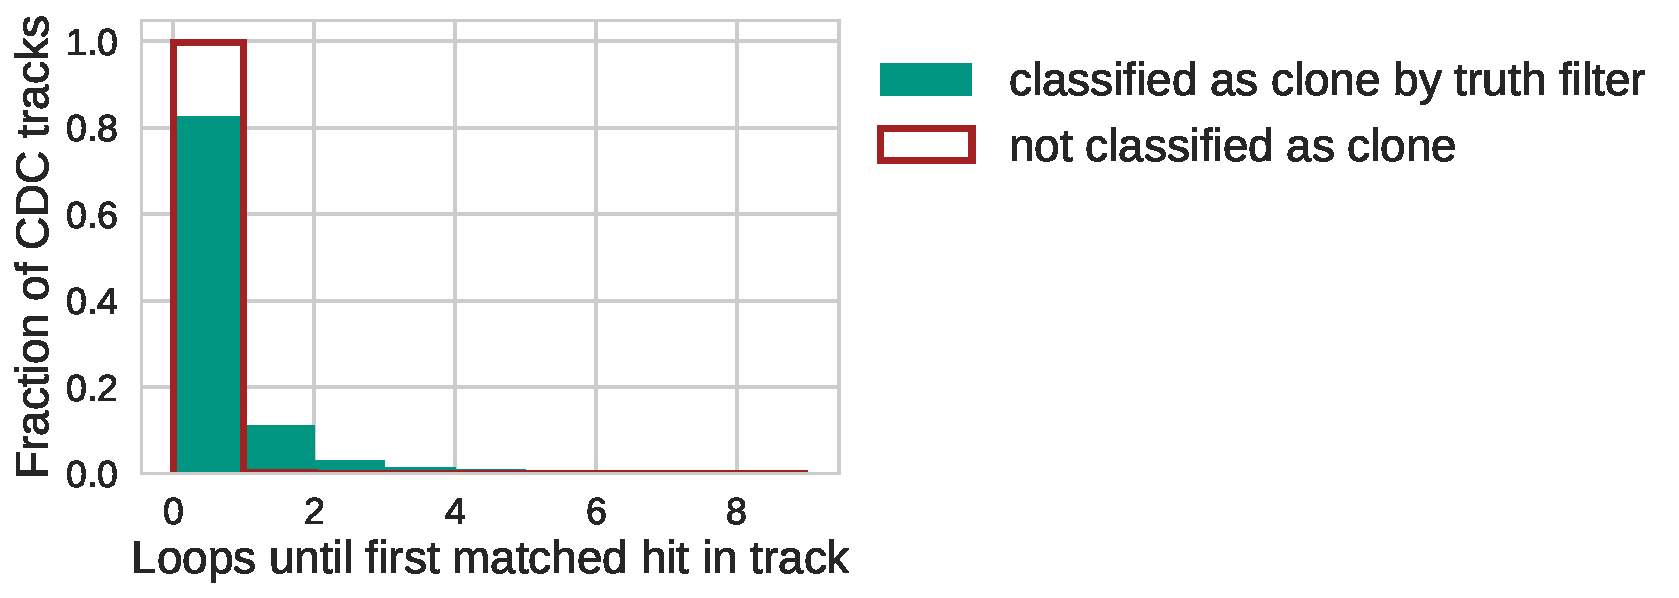
\includegraphics[width=0.7\textwidth]{figures/loop_numbers.pdf}\\
  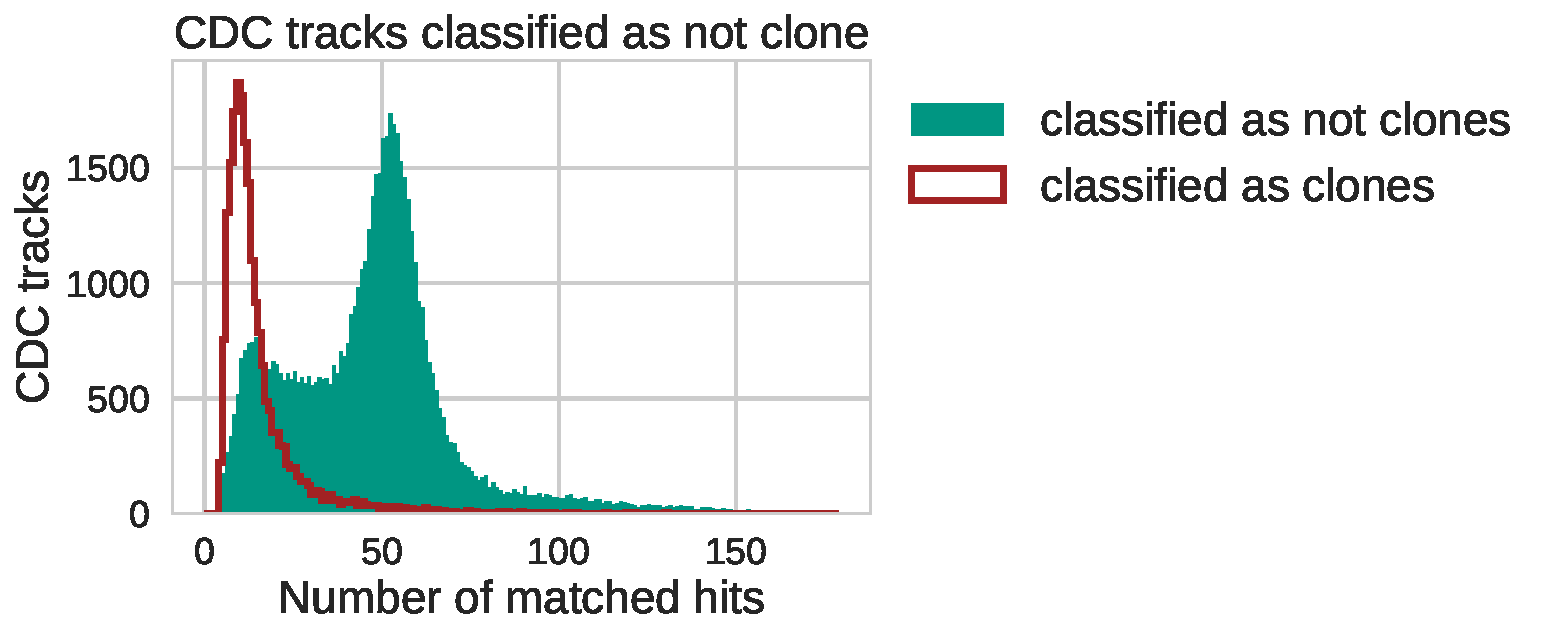
\includegraphics[width=0.7\textwidth]{figures/matched_hits.pdf}\\
\end{frame}

\begin{frame}
  \frametitle{Features currently used for CDC Track Rejecter training}
  As defined in \texttt{tracking/trackFindingCDC/filters/track/BasicTrackVarSet.h}
  \begin{columns}
    \begin{column}{0.5\textwidth}
      \begin{itemize}
      \item \lstinline{size}
      \item \lstinline{pt}
      \item \lstinline{sz_slope}
      \item \lstinline{drift_length_mean}
      \item \lstinline{drift_length_variance}
      \item \lstinline{drift_length_max}
      \item \lstinline{drift_length_min}
      \item \lstinline{drift_length_sum}
      \item \lstinline{adc_mean}
      \item \lstinline{adc_variance}
      \end{itemize}
    \end{column}
    \begin{column}{0.5\textwidth}
      \begin{itemize}

      \item \lstinline{adc_max}
      \item \lstinline{adc_min}
      \item \lstinline{adc_sum}
      \item \lstinline{empty_s_mean}
      \item \lstinline{empty_s_variance}
      \item \lstinline{empty_s_max}
      \item \lstinline{empty_s_min}
      \item \lstinline{empty_s_sum}
      \item \lstinline{has_matching_segment}
      \item \lstinline{s_range}
      \end{itemize}      
    \end{column}
  \end{columns}

\end{frame}

\end{document}

%%% Local Variables:
%%% coding: utf-8
%%% mode: LaTeX
%%% TeX-engine: default
%%% TeX-master: t
%%% ispell-dictionary: "english"
%%% synosaurus-backend: synosaurus-backend-wordnet
%%% fill-column: 100
%%% End:
%%% Local Variables: